\chapter{Online Recognition Evaluation}\label{sec:evaluation}
In the previous sections, I have reported some evaluation results most pertinent
to the sections under discussion. In this chapter, I present results
for the overall online recognition performance.

\section{Evaluation Protocol}
I evaluate the online gesture recognition performance using the YANG
dataset, and the hybrid performance
metrics proposed in Section~\ref{sec:metrics}. The evaluation is based on the
assumption that all the path gestures (gesture \#1--4) are
discrete flow gestures, and pose gestures (gesture \#5--7) are continuous flow
gestures.
The survey results in Section~\ref{sec:preferences} show that it is
important to allow users to quickly define and train their own gestures. Hence,
I evaluate my system using user dependent training and testing. For each user
in the dataset, I use the first 2 sessions of recording (6 samples per gesture)
as training examples, and the last 2 sessions as testing examples. The first 2
sessions have ``Rest'' prompts which help to do automatic segmentation on the
training data.

Figure~\ref{fig:recog-result} shows a visualization of the recognition result on
a test sequence. The figure highlights the challenges in the test sequences:
there are 21 gestures in each continuous unsegmented sequence; sometimes
gestures immediately follow one another.

The average test results for 10 users are reported.

\begin{figure}[thb]
\centering
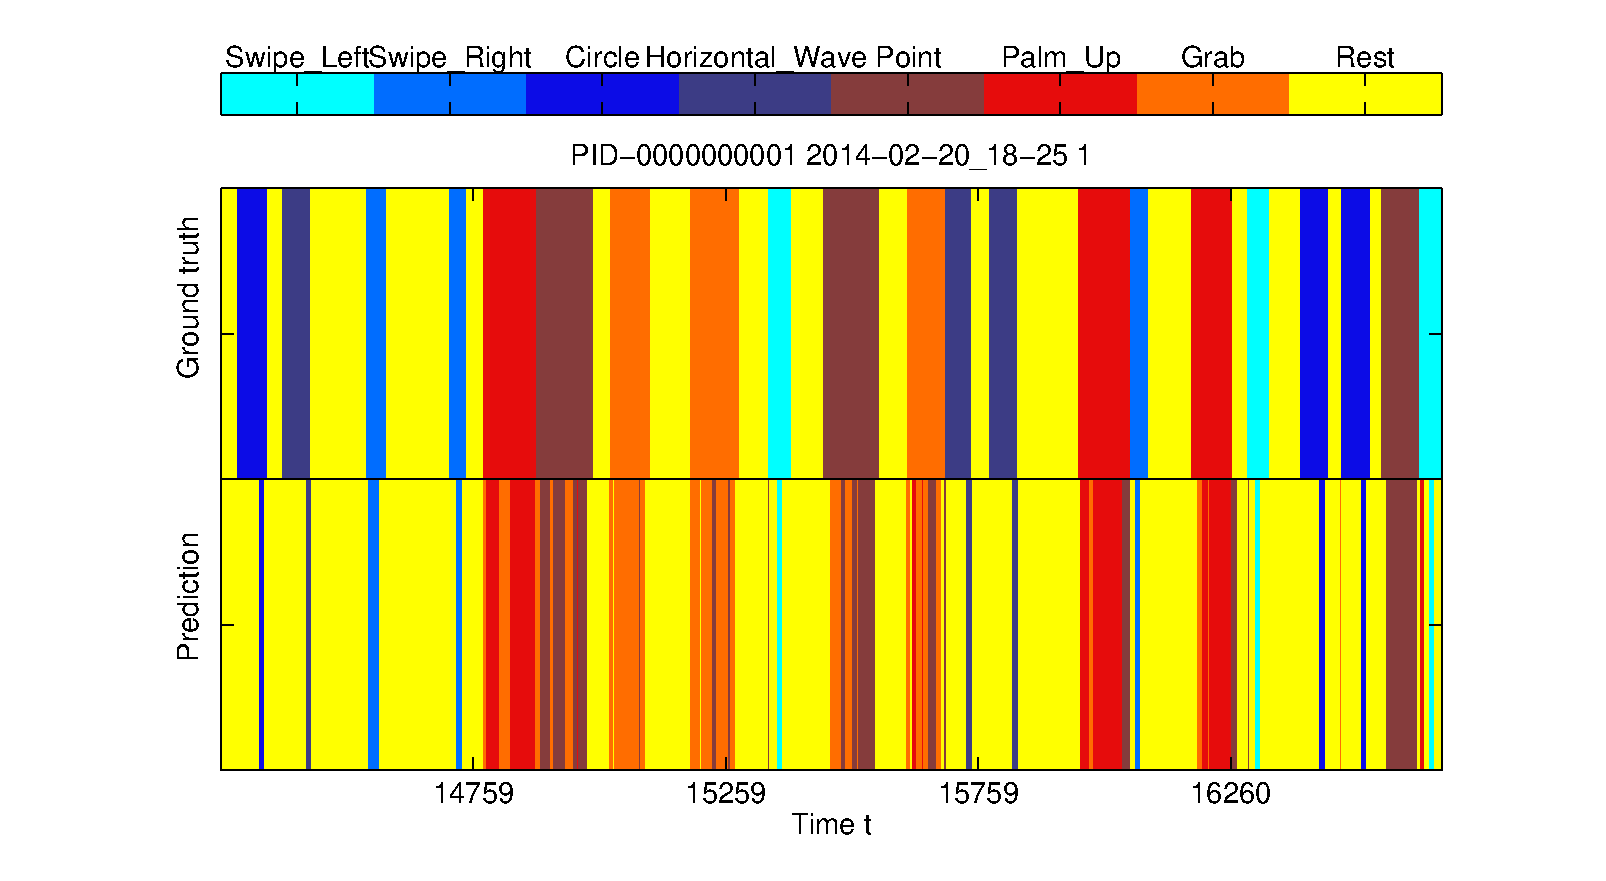
\includegraphics[trim=10mm 5mm 10mm 5mm, clip,
width=\columnwidth]{figures/recog_result_m3.eps}
\caption{Comparison between recognition result using online inference
and ground truth.
The colors correspond to different gestures. For discrete flow gestures
(Swipe Left/Right, Circle, Horizontal Wave), one color segment with a fixed
length is shown at the time of response. For continuous flow gestures, the
recognized gesture is shown at each frame indicating frame-by-frame responses.}
\label{fig:recog-result}
\end{figure}

\section{Compare Different Numbers of Principal Components}
With everything else the same, Figure~\ref{fig:pca} shows the recognition $F_1$
scores with changing number of principal components used for the HOG
descriptor.
The best average score is obtained when 15 principal components are used.

\begin{figure}[tbh]
\centering
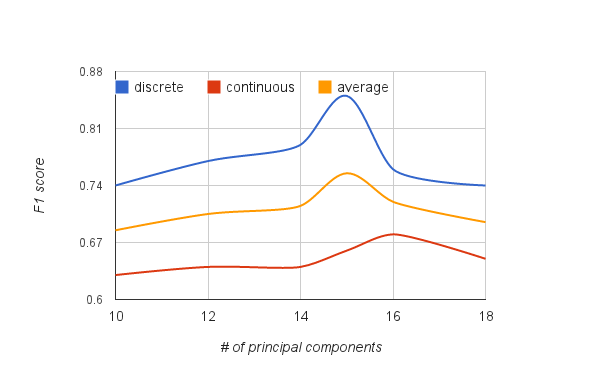
\includegraphics[width=\columnwidth]{figures/f1_pca.png}
\caption{Graph showing how $F_1$ scores for discrete flow gestures, continuous
flow gestures and the average scores change with the number of principal
components used for the HOG descriptor.}
\label{fig:pca}
\end{figure}

\section{Compare Different Topologies}
In this section, I compare my unified framework with a common HMM-based approach
used in previous works~\cite{sharma00, Starner95}, i.e., using the same
left-right topology for all gestures.

Table~\ref{tab:result} compares the results between the two methods.
The third column is the result from treating the two forms of gestures in the
same way, i.e., all gestures have the same left-right Bakis model for their nucleus
phases. The forth column is the result from using a left-right Bakis model for
path gestures and a single state for pose gestures. To have a fair comparison,
all hidden states have 3 mixtures of Gaussians. As Table~\ref{tab:result}
shows, having different HMM topologies for the two forms of gestures significantly increases the recall and $F_1$ score
for pose gestures.

\begin{table}[tbh]
\centering
\begin{tabular}{|l|l|p{3cm}|p{3cm}|}
\hline
& & \textbf{Same topology for two forms of gestures} & \textbf{Different
topologies for two forms of gestures} \\
\hline
\multirow{4}{4cm}{Path \& discrete flow gestures} 
& Precision & \textbf{0.84 (0.16)} & 0.82 (0.16) \\
\cline{2-4}
& Recall & 0.87 (0.17) & 0.87 (0.18)\\
\cline{2-4}
& $F_1$ & \textbf{0.85 (0.16)} &  0.84 (0.16)\\
\cline{2-4}
& Responsiveness (s) & 0.6 (0.3) & 0.6 (0.3) \\
\hline
\multirow{4}{4.5cm}{Pose \& continuous flow gestures}
& Precision & \textbf{0.65 (0.14)} & 0.63 (0.11) \\
\cline{2-4}
& Recall & 0.41 (0.15) & \textbf{0.65 (0.09)} \\
\cline{2-4}
& $F_1$ & 0.50(0.14) & \textbf{0.64 (0.10)} \\
\hline
\textbf{Average} & $F_1$ & 0.675 (0.150) & \textbf{0.740 (0.130)} \\
\hline
\end{tabular}
\caption{Results from using different topologies. The numbers in parentheses are
standard deviations. The results are based on using 3 mixtures of Gaussians
for all hidden states, and lag time
$l = 8$ frames.}
\label{tab:result}
\end{table}

For gestures with arbitrary movement (e.g., pose gestures), it is difficult to
use embedded training to accurately align pre-stroke, nucleus and post-stroke phases.
Figure~\ref{fig:palm-hidden} illustrates this problem. It shows the most
likely hidden state estimates for a Palm Up gesture sequence. The main (center)
part of the gesture, which should be the nucleus of the gesture, is identified
as the post-stroke. This is why it is important to have different topologies and
different training strategies for the two forms of gestures.

\begin{figure}[tbh]
\centering
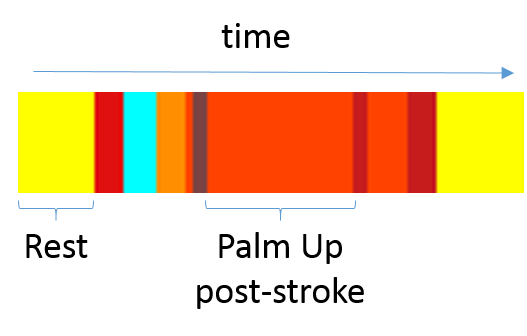
\includegraphics[width=0.3\linewidth]{figures/palm_hidden_label.png}
\caption{Estimated hidden states for a ``Palm Forward'' gesture using the
left-right model same as gestures with distinct path. Different colors correspond to
different hidden states.}
\label{fig:palm-hidden}
\end{figure}

\section{Compare Different Numbers of Mixtures}
The previous section shows that using different topologies for path and pose
gestures give better
recognition performance. So using this model, I investigate the effects
of the number of mixtures ($k$) in the MoG emission probabilities.

First, I set $k$ be the same for both forms of gestures.
Fig.~\ref{fig:mixtures} shows that the $F_1$ scores increases as the number of
mixtures increases until $k=3$.
After that, we start to see the effect of overfitting.

\begin{figure}[tbh]
\centering
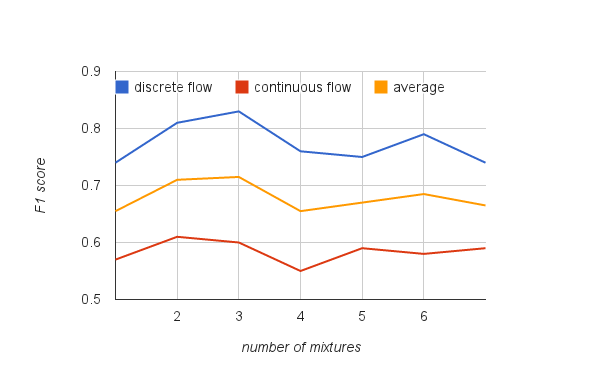
\includegraphics[trim=10mm 5mm 10mm 15mm,
clip, width=\columnwidth]{figures/f1_nM.png}
\caption{F1 scores versus number of mixtures.}
\label{fig:mixtures}
\end{figure}

Then, I experimented with using different $k$'s for path and pose gestures. I
set $k^\text{path} = 3$ for path gestures, and use a different
$k^{\text{pose}}_g\in \{3\ldots6\}$ for pose gesture $g$. Each
$k^{\text{pose}}_g$ is chosen according to Section~\ref{sec:pose-gesture}.
Using this method, I am able to improve precision, recall and $F_1$ scores for
both forms of the gestures even further (see
Table~\ref{tab:different-mixtures}).

\begin{table}[tbh]
\centering
\begin{tabular}{|p{4.5cm}|l|p{4cm}|}
\hline
& & \textbf{Use different topologies and numbers of mixtures} \\
\hline
\multirow{4}{4cm}{Path \& discrete flow gestures} 
& Precision & \textbf{0.94 (0.05)} \\
\cline{2-3}
& Recall    & \textbf{0.93 (0.08)} \\
\cline{2-3}
& $F_1$ & \textbf{0.93 (0.06)} \\
\cline{2-3}
& Responsiveness (s) & 0.6 (0.2)  \\
\hline
\multirow{3}{4cm}{Pose \& continuous flow gestures}
& Precision & \textbf{0.68 (0.10)} \\
\cline{2-3}
& Recall & \textbf{0.69 (0.08)} \\
\cline{2-3}
& $F_1$ & \textbf{0.68 (0.09)}  \\
\hline
\textbf{Average} & $F_1$ & \textbf{0.805 (0.075)}\\
\hline
\end{tabular}
\caption{Results from using different numbers of mixtures of Gaussians
for the emission probabilities ($l = 8$ frames).}
\label{tab:different-mixtures}
\end{table}

%Compare user dependent vs user independent result

\section{Compare Different Lag Times}
Figure\ref{fig:lag} shows how the $F_1$ scores change with respect to the lag
time ($l$) in fixed-lag smoothing. The performance increases as $l$ increases, and
plateaus at $l=8$ frames which is about 0.3s at 30 FPS. This shows that more
evidence does help to smooth the estimates until a limit, and we do not need to
sacrifice too much delay to reach the limit. Our result also shows that the
responsiveness score stays around 0.6--0.7 seconds as $l$ is increased.

\begin{figure}[!tbh]
\centering
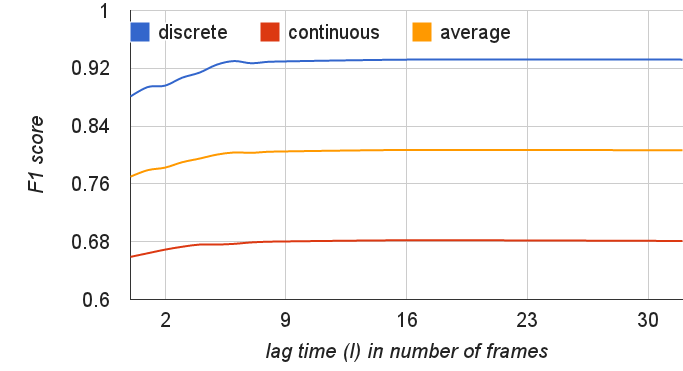
\includegraphics[trim=0 5mm 0 15mm, clip,
width=\columnwidth]{figures/f1_lag.png}
\caption{$F_1$ scores versus lag time $l$.}
\label{fig:lag}
\end{figure}

\section{Training Time}
The HMM-based unified framework is fast to train as well. The average
computation time for training the model for one user is about 5s with 7 gestures and 6 training examples per
gesture. 

\section{User Independent Evaluation}
The survey (Section~\ref{sec:preferences}) indicates that users
generally prefer a system to have a predefined gesture set and then add or
change gestures later according to their own preferences. This means that having
a user independent base model will be useful as well. If the system has user
provided training examples for certain gestures, it uses the
user dependent models for those gestures; otherwise it backs off the the base
model. This adaptation strategy is similar to~\cite{yin13-making}.

To evaluate the user independent model, I did a 10-fold cross-validation where
in each fold, the data from one user's last 2 sessions are used for testing and
the data from the remaining 9 users' first 2 sessions are used for training.
Table~\ref{tab:user-independent} shows the average, best and worst results among
the users. We can see that there is large variation among the users. For users
who want to the gestures differently, they need to train their user independent
models. For example, the results based on user dependen model for user PID-02 is
much better than the user independent model.

\begin{table}[tbh]
\centering
\begin{tabular}{|p{3cm}|l|l|p{1.9cm}|p{1.9cm}||p{2cm}|}
\hline
& & \textbf{Average} & \textbf{Best (PID-01)} & \textbf{Worst (PID-02)} &
\textbf{User dep. (PID-02)} \\
\hline
\multirow{4}{3cm}{Path \& discrete flow gestures} 
& Precision & 0.72 (0.18) & 1.00 & 0.35 & 0.96 \\
\cline{2-6}
& Recall    & 0.72 (0.16) & 1.00 & 0.72 & 1.00\\
\cline{2-6}
& $F_1$ & 0.70 (0.16) & 1.00 & 0.47 & 0.98 \\
\cline{2-6}
& Responsiveness (s) & 0.6 (0.3)  & 0.6 & 0.4 &  0.4\\
\hline
\multirow{3}{3cm}{Pose \& continuous flow gestures}
& Precision & 0.59 (0.12) & 0.79 & 0.49 & 0.67\\
\cline{2-6}
& Recall & 0.56 (0.16) & 0.77 & 0.21 & 0.67\\
\cline{2-6}
& $F_1$ & 0.56 (0.13)  & 0.78 & 0.29 & 0.67\\
\hline
\textbf{Average} & $F_1$ & 0.63 (0.15) & 0.89 & 0.38 & 0.83\\
\hline
\end{tabular}
\caption{User independent model 10-fold cross validation results ($l = 8$
frames). The last column is the user dependent result for user PID-02 for
comparison.}
\label{tab:user-independent}
\end{table}

\section{Discussion}
Our overall best performance for the YANG dataset is reported in
Table~\ref{tab:different-mixtures}. The performance for the pose and
continuous flow gestures is relatively low compared to that of the path and
discrete flow gestures. Most
confusions are among the 3 pose gestures, i.e., Point, Palm Up, Grab (see
Figure~\ref{fig:recog-result} for example).
There are big variations in the recognition results for the pose gestures among users: the highest $F_1$ score for pose gestures is 0.81
and the lowest is 0.58. For the ones with low $F_1$ scores, confusion occurs
when there is significant motion blur (see Figure~\ref{fig:point_grab}). These
correspond to the users who move relatively fast when doing the pose gestures.
This suggests that with the frame rate of the Kinect sensor used (30Hz for
the Kinect version one), users may need to perform pose gestures relatively
slowly in order to get better recognition results.

\begin{figure}[tbh]
\centering
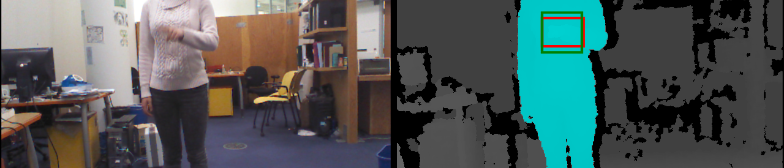
\includegraphics[width=\linewidth]{figures/point_posture_full_image.png}
\caption{This frame is mistakenly classified as Grab while the true gesture
is Point. Motion blur is significant.}
\label{fig:point_grab}
\end{figure}